% Copyright 2018 Melvin Eloy Irizarry-Gelpí
\chapter{Working with Spreadsheets}
%%%%%%%%%%%%%%%%%%%%%%%%%%%%%%%%%%%%%%%%%%%%%%%%%%%%%%%%%%%%%%%%%%%%%%%%%%%%%%%%
In this experiment you will gain experience using spreadsheets to analyze and visualize data.
%%%%%%%%%%%%%%%%%%%%%%%%%%%%%%%%%%%%%%%%%%%%%%%%%%%%%%%%%%%%%%%%%%%%%%%%%%%%%%%%
\section{Preliminary}
%%%%%%%%%%%%%%%%%%%%%%%%%%%%%%%%%%%%%%%%%%%%%%%%%%%%%%%%%%%%%%%%%%%%%%%%%%%%%%%%
Spreadsheet technology is commonly available in the form of software like Microsoft Excel, LibreOffice Calc, or Google Sheets.

Excel is part of Microsoft Office, and you usually need a license to use it. Calc is part of LibreOffice, which is a free version of Microsoft Office. Both Excel and Calc can be used as apps in your desktop or laptop. Google Sheets is very similar, but can be used through a web browser like Chrome or Firefox. All three share a common set of basic functionality, which is what we will need.

Since Google Sheets is available as part of the suit of apps provided by the College, and it works the same way in Windows, Mac OS X, and Linux, I will be using Google Sheets for all my analysis work. Use of Google Sheets is not mandatory but strongly encouraged.

In this experiment you will get a first encounter with using spreadsheets to analyze physics data. You will
\begin{enumerate}
    \item Import data into a spreadsheet
    \item Separate data into distinct measurements
    \item Make charts for visualization
    \item Use built-in functions to analyze the data
    \item Make a table with results
\end{enumerate}
Let us dive in.
%%%%%%%%%%%%%%%%%%%%%%%%%%%%%%%%%%%%%%%%%%%%%%%%%%%%%%%%%%%%%%%%%%%%%%%%%%%%%%%%
\section{Experiment}
%%%%%%%%%%%%%%%%%%%%%%%%%%%%%%%%%%%%%%%%%%%%%%%%%%%%%%%%%%%%%%%%%%%%%%%%%%%%%%%%
There is no actual experiment to collect the data. You will work with two data files, each describing a different hypothetical experiment. Although the data in each file was generated with a computer program, it is similar to some of the data that you will collect later in the semester from sensors during an experiment.
%%%%%%%%%%%%%%%%%%%%%%%%%%%%%%%%%%%%%%%%%%%%%%%%%%%%%%%%%%%%%%%%%%%%%%%%%%%%%%%%
\subsection{Weight Measurement}
%%%%%%%%%%%%%%%%%%%%%%%%%%%%%%%%%%%%%%%%%%%%%%%%%%%%%%%%%%%%%%%%%%%%%%%%%%%%%%%%
This experiment consists of a hypothetical \textbf{weight} measurement taken over \textbf{time}. Three weight values are measured. First, between the starting time $t = t_{I}$ and $t = t_{1}$ a \textbf{baseline weight} measurement $W_{B}$ is taken to calibrate the sensor. Then, between $t = t_{1}$ and $t = t_{2}$ the \textbf{weight 1} measurement $W_{1}$ is taken. Finally, between $t = t_{2}$ and $t = t_{F}$ the \textbf{weight 2} measurement $W_{2}$ is taken. That is:
\begin{itemize}
    \item $t_{I} < t < t_{1}$: Baseline weight measurement $W_{B}$
    \item $t_{1} < t < t_{2}$: Weight 1 measurement $W_{1}$
    \item $t_{2} < t < t_{F}$: Weight 2 measurement $W_{2}$
\end{itemize}
You need to provide the best estimate for the three weight values from the data.

Although this is a measurement over time, we will treat each time measurement as \textbf{independent}. That is, this hypothetical sensor is repeatedly measuring the same quantity, but due to noise, it cannot provide the same result each time. The main challenge is to deal with this noise. Which value to report? The first one? The last one? The one in the middle of the experiment? One value chosen at random?
%%%%%%%%%%%%%%%%%%%%%%%%%%%%%%%%%%%%%%%%%%%%%%%%%%%%%%%%%%%%%%%%%%%%%%%%%%%%%%%%
\subsection{Velocity Measurement}
%%%%%%%%%%%%%%%%%%%%%%%%%%%%%%%%%%%%%%%%%%%%%%%%%%%%%%%%%%%%%%%%%%%%%%%%%%%%%%%%
This experiment consist of a hypothetical \textbf{velocity} measurement taken over \textbf{time}. You need to see if there exist a relationship between the velocity values and the time values. In order to answer this, it will be helpful to make a chart of velocity versus time.
%%%%%%%%%%%%%%%%%%%%%%%%%%%%%%%%%%%%%%%%%%%%%%%%%%%%%%%%%%%%%%%%%%%%%%%%%%%%%%%%
\section{Analysis}
%%%%%%%%%%%%%%%%%%%%%%%%%%%%%%%%%%%%%%%%%%%%%%%%%%%%%%%%%%%%%%%%%%%%%%%%%%%%%%%%
There are two separate parts. But before the analysis you need to setup your environment.
%%%%%%%%%%%%%%%%%%%%%%%%%%%%%%%%%%%%%%%%%%%%%%%%%%%%%%%%%%%%%%%%%%%%%%%%%%%%%%%%
\subsection{Setup for Weight Measurement}
%%%%%%%%%%%%%%%%%%%%%%%%%%%%%%%%%%%%%%%%%%%%%%%%%%%%%%%%%%%%%%%%%%%%%%%%%%%%%%%%
Here are some steps to follow before you can analyze the weight data.
%%%%%%%%%%%%%%%%%%%%%%%%%%%%%%%%%%%%%%%%%%%%%%%%%%%%%%%%%%%%%%%%%%%%%%%%%%%%%%%%
\subsubsection{Obtain the data}
%%%%%%%%%%%%%%%%%%%%%%%%%%%%%%%%%%%%%%%%%%%%%%%%%%%%%%%%%%%%%%%%%%%%%%%%%%%%%%%%
This step involves obtaining the data. For this activity, I will provide you with data. Later in the semester you will collect your own data from an experiment!

You can find the data file \texttt{weight.tsv} in Canvas. Download the file and add it to your working directory (either in your own computer or to your Google Drive in the cloud). It is a good idea to organize your files by lab number, so this data file could be inside a folder named \texttt{lab-00-intro}.

The file extension \texttt{.tsv} means \textbf{Tab-Separated Values}, meaning that each line consist of values separated by tab spaces. The files generated by the Vernier data collection devices that we are going to use will be in a similar format, but will have a file extension \texttt{.txt} for \textbf{Plain Text}. Both formats can be used with Google Sheets.
%%%%%%%%%%%%%%%%%%%%%%%%%%%%%%%%%%%%%%%%%%%%%%%%%%%%%%%%%%%%%%%%%%%%%%%%%%%%%%%%
\subsubsection{View the data}
%%%%%%%%%%%%%%%%%%%%%%%%%%%%%%%%%%%%%%%%%%%%%%%%%%%%%%%%%%%%%%%%%%%%%%%%%%%%%%%%
This step is a sanity check: you want to take a \textbf{quick glimpse} at the data that you just obtained to make sure that everything is going well.

You can use a simple \textbf{text editor} like Notepad (Windows) or TextEdit (Mac OS X) to open and view the data. You should see about 600 lines of text, each with two numerical values. The first line is a \textbf{header} and contains information about the data below. In our case, the header says that the first column is a quantity representing \textbf{time} measured in \textbf{seconds} (s), and the second column is a quantity representing \textbf{weight} measured in \textbf{pounds} (lb). Both the \textbf{names} and the \textbf{units} of each quantity are equally important.

Note that Microsoft Word and/or Google Docs are not simple text editors but complicated \textbf{word processors}. A text editor only allows simple editing like adding, changing, or removing characters in a text. A word processor allows you to format a text into different pages, make text bold, change fonts, etcetera. If you use a word processor to view data, the data will get split into multiple pages, and also might acquire unnecessary formating.

As you can see, a single data file with hundreds of rows can correspond to dozens of pages of paper. For this reason, \textbf{you should not include raw data files in your lab reports}. It is more useful (and less wasteful) to include the raw data in a spreadsheet that is shared electronically.
%%%%%%%%%%%%%%%%%%%%%%%%%%%%%%%%%%%%%%%%%%%%%%%%%%%%%%%%%%%%%%%%%%%%%%%%%%%%%%%%
\subsubsection{Start a new spreadsheet}
%%%%%%%%%%%%%%%%%%%%%%%%%%%%%%%%%%%%%%%%%%%%%%%%%%%%%%%%%%%%%%%%%%%%%%%%%%%%%%%%
It goes without saying that you should begin with an \textbf{empty spreadsheet}. Please, give your spreadsheet a useful \textbf{file name} so that it can be later identified and distinguished from spreadsheets from other students, and from your own spreadsheets from other experiments. For example, \texttt{irizarry-gelpi-lab-00} is a good file name because:
\begin{itemize}
    \item \texttt{irizarry-gelpi} indicates the \textbf{name} of the owner of the spreadsheet
    \item \texttt{lab-00} indicates which \textbf{experiment} is in the spreadsheet
\end{itemize}
Each student is required to submit a spreadsheet. There is no need to include your partner's name. Also, no need to include information about the version like \texttt{v1} or \texttt{final}.

Do not submit a file called \texttt{physics-lab} or \texttt{Untitled spreadsheet}. Students who do not follow this practice will get points taken off.
%%%%%%%%%%%%%%%%%%%%%%%%%%%%%%%%%%%%%%%%%%%%%%%%%%%%%%%%%%%%%%%%%%%%%%%%%%%%%%%%
\subsubsection{Import the data}
%%%%%%%%%%%%%%%%%%%%%%%%%%%%%%%%%%%%%%%%%%%%%%%%%%%%%%%%%%%%%%%%%%%%%%%%%%%%%%%%
This step involves putting the data into Google Sheets or Excel for analysis.

If you \textbf{copy and paste} the data directly into a spreadsheet, you will probably end with a \textbf{single column} of data. But if you look closely, the data involves two columns of numbers. A single column with spaced values is not useful in a spreadsheet.

Instead of copying and pasting the data, it is better to \textbf{import} it. In Google Sheets, you can do this by going to
\begin{center}
    \texttt{File > Import}
\end{center}
Find your file. As import location, choose \texttt{Insert new sheet(s)}. You do not need to change any other import setting. After this you should see a spreadsheet with \textbf{two columns} of data. Column \texttt{A} should be time, and column \texttt{B} should be weight.

I will refer to this sheet with the raw data by the name \texttt{RawData}. You can change the name of a sheet by double-clicking on the tab near the bottom of the screen.
%%%%%%%%%%%%%%%%%%%%%%%%%%%%%%%%%%%%%%%%%%%%%%%%%%%%%%%%%%%%%%%%%%%%%%%%%%%%%%%%
\subsubsection{Visualize the full data}
%%%%%%%%%%%%%%%%%%%%%%%%%%%%%%%%%%%%%%%%%%%%%%%%%%%%%%%%%%%%%%%%%%%%%%%%%%%%%%%%
This step involves making a chart in order to obtain an initial visualization of the full data.

Before any analysis is done on the new data, it is always useful to make a quick visualization. You can do this by selecting the two columns with data (hold the \texttt{Shift} key), and clicking on \texttt{Insert Chart}. By default, Google Sheets will provide you with a \textbf{line chart}. This is not necessarily the best option for our kind of data, so change the \texttt{Chart Type} to a \textbf{scatter chart}. You will get a chart with points instead of a line. I find it convenient to change the default settings for the size of the points, in order to obtain a better graph. You can double-click on a chart to access the \texttt{Chart editor} menu, and then going to
\begin{center}
    \texttt{Chart Editor > Customize > Series > Point Size}
\end{center}
and changing the value from \texttt{7px} to \texttt{2px}.

You should see three horizontal regions with points. Each region corresponds to a different measurement. Looking at the graph you can learn that
\begin{itemize}
    \item The baseline weight measurement happens between $t = 0$ s and $t = 10$ s
    \item The weight 1 measurement happens between $t = 10$ s and $t = 20$ s
    \item The weight 2 measurement happens between $t = 20$ s and $t = 30$ s
\end{itemize}
By just looking at the graph, you have already learned something useful about the data.
%%%%%%%%%%%%%%%%%%%%%%%%%%%%%%%%%%%%%%%%%%%%%%%%%%%%%%%%%%%%%%%%%%%%%%%%%%%%%%%%
\subsubsection{Separate the data}
%%%%%%%%%%%%%%%%%%%%%%%%%%%%%%%%%%%%%%%%%%%%%%%%%%%%%%%%%%%%%%%%%%%%%%%%%%%%%%%%
Since there are three different measurements, it would be useful to work on three \textbf{separate sheets}. Add three empty sheets and give them useful names like \texttt{Baseline}, \texttt{One}, and \texttt{Two} or something similar that will help you remember later what each sheet corresponds to.

The first row on each sheet should be a header with the name and unit of each quantity. You can copy and paste the header row in \texttt{RawData}. The sheet with the baseline measurement should have the data between times 0 s and 10 s. You can select this region in \texttt{RawData}, copy it, and paste it to the \texttt{Baseline} sheet. Note that the baseline measurement actually ends at the 9.95 s time value. After doing this, the \texttt{Baseline} sheet should have about 200 rows with data. Similar steps can be taken with the other two measurements.
%%%%%%%%%%%%%%%%%%%%%%%%%%%%%%%%%%%%%%%%%%%%%%%%%%%%%%%%%%%%%%%%%%%%%%%%%%%%%%%%
\subsubsection{Visualize each segment}
%%%%%%%%%%%%%%%%%%%%%%%%%%%%%%%%%%%%%%%%%%%%%%%%%%%%%%%%%%%%%%%%%%%%%%%%%%%%%%%%
After separating each segment, it will be helpful to make a scatter chart for each portion, in order to get a better idea of how each segment looks up close.

Each chart should have a \textbf{title}, and \textbf{labeled horizontal and vertical axes}. You can double-click on a chart to access the \texttt{Chart editor} menu. The title can be changed under
\begin{center}
    \texttt{Chart editor > Chart \& axis titles > Type}
\end{center}
and choose the \texttt{Chart title} option to add a title to the chart. A good title would be something along the lines of ``Baseline Measurement'' in order to provide context. You can add a label to the horizontal axis by choosing \texttt{Horizontal axis title} instead. A good axis label will include the \textbf{name of the quantity} and the \textbf{units} being used to measure it. For example, ``Time (s)'' and ``Weight (lb)''.

Other useful changes to the default settings are to reduce the size of the points, and to remove the legend, since only one quantity is being plotted.
%%%%%%%%%%%%%%%%%%%%%%%%%%%%%%%%%%%%%%%%%%%%%%%%%%%%%%%%%%%%%%%%%%%%%%%%%%%%%%%%
\subsubsection{Use named ranges}
%%%%%%%%%%%%%%%%%%%%%%%%%%%%%%%%%%%%%%%%%%%%%%%%%%%%%%%%%%%%%%%%%%%%%%%%%%%%%%%%
You are going to use the data in the spreadsheet to calculate quantities that are going to help you understand and describe the data. In order to do these calculations, it will be convenient to give nicknames to the parts of the spreadsheet with the numerical weight data. These are called \textbf{named ranges}. To add a named range, first open the menu by going to
\begin{center}
    \texttt{Data > Named ranges...}
\end{center}
Go to the \texttt{Baseline} sheet, and select the second cell in the weight column (i.e. the first cell with a numerical value in column \texttt{B}). Hold the \texttt{Shift} key and press the \texttt{Page Down} key or down arrow key to move down along the column all the way to the end. When all the numerical values in that column are selected, click on \texttt{+ Add a range} and give it a useful name like \texttt{WeightB} (for baseline weight). Finally, click on \texttt{Done}. You can do something similar for the weight column in the other two segments.
%%%%%%%%%%%%%%%%%%%%%%%%%%%%%%%%%%%%%%%%%%%%%%%%%%%%%%%%%%%%%%%%%%%%%%%%%%%%%%%%
\subsubsection{Significant Figures}
%%%%%%%%%%%%%%%%%%%%%%%%%%%%%%%%%%%%%%%%%%%%%%%%%%%%%%%%%%%%%%%%%%%%%%%%%%%%%%%%
Take a look at the numbers in both the time and weight columns. The time column contains values with at most 2 decimal figures. For the weight column, the values have at most 6 decimal figures. This means that any time quantity that we compute should be rounded to 2 decimal places, and any weight quantity should be rounded to 6 decimal places.
%%%%%%%%%%%%%%%%%%%%%%%%%%%%%%%%%%%%%%%%%%%%%%%%%%%%%%%%%%%%%%%%%%%%%%%%%%%%%%%%
\subsection{Descriptive Statistics for Weight Measurement}
%%%%%%%%%%%%%%%%%%%%%%%%%%%%%%%%%%%%%%%%%%%%%%%%%%%%%%%%%%%%%%%%%%%%%%%%%%%%%%%%
The steps in this section apply to each of the three segments in the data, but \textbf{I will use the baseline segment} for illustration purposes.
%%%%%%%%%%%%%%%%%%%%%%%%%%%%%%%%%%%%%%%%%%%%%%%%%%%%%%%%%%%%%%%%%%%%%%%%%%%%%%%%
\subsubsection{Minimum}
%%%%%%%%%%%%%%%%%%%%%%%%%%%%%%%%%%%%%%%%%%%%%%%%%%%%%%%%%%%%%%%%%%%%%%%%%%%%%%%%
Since the weight values are spread over a region, it is useful to known what is the smallest weight measurement in the segment, also known as the \textbf{minimum}. One way to do this is to literally scan the weight column and keep track of the smallest value. That is not a good idea when you have hundreds of values. A more efficient way is to have Google Sheets do this for you. The minimum can be found by using the \texttt{MIN} function via
\begin{center}
    \texttt{=MIN(WeightB)}
\end{center}
Note the equal sign in the beginning. In my case, the minimum weight value in the baseline segment is 3.468206 lb.
%%%%%%%%%%%%%%%%%%%%%%%%%%%%%%%%%%%%%%%%%%%%%%%%%%%%%%%%%%%%%%%%%%%%%%%%%%%%%%%%
\subsubsection{25th Percentile}
%%%%%%%%%%%%%%%%%%%%%%%%%%%%%%%%%%%%%%%%%%%%%%%%%%%%%%%%%%%%%%%%%%%%%%%%%%%%%%%%
The \textbf{25th percentile} is the weight value measured that is larger than one quarter of all of the weight values in the data. This can be computed using the \texttt{PERCENTILE} function via
\begin{center}
    \texttt{=PERCENTILE(WeightB, 0.25)}
\end{center}
Equivalently, this can be computed using the \texttt{QUARTILE} function via
\begin{center}
    \texttt{=QUARTILE(WeightB, 1)}
\end{center}
The ``1'' here indicates the \textbf{first quartile}, which is another name for the 25th percentile. In my case, the 25th percentile in the baseline segment is 4.57650975 lb. That is, about a quarter of the weight measurements are smaller than 4.576510 lb.
%%%%%%%%%%%%%%%%%%%%%%%%%%%%%%%%%%%%%%%%%%%%%%%%%%%%%%%%%%%%%%%%%%%%%%%%%%%%%%%%
\subsubsection{50th Percentile}
%%%%%%%%%%%%%%%%%%%%%%%%%%%%%%%%%%%%%%%%%%%%%%%%%%%%%%%%%%%%%%%%%%%%%%%%%%%%%%%%
The \textbf{50th percentile} (also known as the \textbf{median}) is the weight value measured that is larger than one half of all the weight values in the data. This can be computed using the \texttt{PERCENTILE} function via
\begin{center}
    \texttt{=PERCENTILE(WeightB, 0.50)}
\end{center}
Equivalently, this can be computed using the \texttt{QUARTILE} function via
\begin{center}
    \texttt{=QUARTILE(WeightB, 2)}
\end{center}
The ``2'' here indicates the \textbf{second quartile}. You can also use the \texttt{MEDIAN} function via
\begin{center}
    \texttt{=MEDIAN(WeightB)}
\end{center}
All three functions will return the same value. In my case, the 50th percentile in the baseline segment is 5.032499 lb.
%%%%%%%%%%%%%%%%%%%%%%%%%%%%%%%%%%%%%%%%%%%%%%%%%%%%%%%%%%%%%%%%%%%%%%%%%%%%%%%%
\subsubsection{75th Percentile}
%%%%%%%%%%%%%%%%%%%%%%%%%%%%%%%%%%%%%%%%%%%%%%%%%%%%%%%%%%%%%%%%%%%%%%%%%%%%%%%%
The \textbf{75th percentile} is the weight value measured that is larger than three quarters of all of the weight values in the data. This can be computed using the \texttt{PERCENTILE} function via
\begin{center}
    \texttt{=PERCENTILE(WeightB, 0.75)}
\end{center}
Equivalently, this can be computed using the \texttt{QUARTILE} function via
\begin{center}
    \texttt{=QUARTILE(WeightB, 3)}
\end{center}
The ``3'' here indicates the \textbf{third quartile}. In my case, the 75th percentile in the baseline segment is 5.484631 lb. That is, about 3/4 of the weight measurements are smaller than 5.484631 lb.
%%%%%%%%%%%%%%%%%%%%%%%%%%%%%%%%%%%%%%%%%%%%%%%%%%%%%%%%%%%%%%%%%%%%%%%%%%%%%%%%
\subsubsection{Maximum}
%%%%%%%%%%%%%%%%%%%%%%%%%%%%%%%%%%%%%%%%%%%%%%%%%%%%%%%%%%%%%%%%%%%%%%%%%%%%%%%%
The \textbf{maximum} is the largest weight value recorded. You can find this by using the \texttt{MAX} function:
\begin{center}
    \texttt{=MAX(WeightB)}
\end{center}
In my case, the maximum weight value in the baseline segment is 6.429887 lb.
%%%%%%%%%%%%%%%%%%%%%%%%%%%%%%%%%%%%%%%%%%%%%%%%%%%%%%%%%%%%%%%%%%%%%%%%%%%%%%%%
\subsubsection{Average}
%%%%%%%%%%%%%%%%%%%%%%%%%%%%%%%%%%%%%%%%%%%%%%%%%%%%%%%%%%%%%%%%%%%%%%%%%%%%%%%%
So far we have identified particular points in the data that have special significance: the min, quartiles, and max. The \textbf{average}, also known as the \textbf{arithmetic mean}, or just the \textbf{mean}, is another value that can be calculated from the data, but that in general does not correspond to any point in the data. The average can be interpreted as a sort of ``middle'' or ``typical'' value. You can calculate this with the \texttt{AVERAGE} function:
\begin{center}
    \texttt{=AVERAGE(WeightB)}
\end{center}
Mathematically, given $N$ values of weight $w_{1}$, $w_{2}$, ..., $w_{N}$, the arithmetic mean weight $w_{A}$ is given by
\begin{equation}
    w_{A} = \frac{1}{N} \left( w_{1} + w_{2} + ... + w_{N} \right)
\end{equation}
In my case, the average weight value in the baseline segment is 5.042546 lb. Note that this is different from the median.
%%%%%%%%%%%%%%%%%%%%%%%%%%%%%%%%%%%%%%%%%%%%%%%%%%%%%%%%%%%%%%%%%%%%%%%%%%%%%%%%
\subsubsection{Geometric Mean}
%%%%%%%%%%%%%%%%%%%%%%%%%%%%%%%%%%%%%%%%%%%%%%%%%%%%%%%%%%%%%%%%%%%%%%%%%%%%%%%%
Besides the traditional average used above, there are many other kinds of averages that can be computed. The \textbf{geometric mean} is another one that can be conveniently computed with the \texttt{GEOMEAN} function:
\begin{center}
    \texttt{=GEOMEAN(WeightB)}
\end{center}
Mathematically, given $N$ values of weight $w_{1}$, $w_{2}$, ..., $w_{N}$, the geometric mean weight $w_{G}$ is given by
\begin{equation}
    w_{G} = \left( w_{1} \times w_{2} \times ... \times w_{N} \right)^{1/N}
\end{equation}
In my case, the geometric mean weight value in the baseline segment is 5.005110 lb.
%%%%%%%%%%%%%%%%%%%%%%%%%%%%%%%%%%%%%%%%%%%%%%%%%%%%%%%%%%%%%%%%%%%%%%%%%%%%%%%%
\subsubsection{Harmonic Mean}
%%%%%%%%%%%%%%%%%%%%%%%%%%%%%%%%%%%%%%%%%%%%%%%%%%%%%%%%%%%%%%%%%%%%%%%%%%%%%%%%
The \textbf{harmonic mean} is yet another kind of average that can be conveniently computed with the \texttt{HARMEAN} function:
\begin{center}
    \texttt{=HARMEAN(WeightB)}
\end{center}
Mathematically, given $N$ values of weight $w_{1}$, $w_{2}$, ..., $w_{N}$, the harmonic mean weight $w_{H}$ is given by
\begin{equation}
    w_{H} = N \left( \frac{1}{w_{1}} + \frac{1}{w_{2}} + ... + \frac{1}{w_{N}} \right)^{-1}
\end{equation}
In my case, the harmonic mean weight value in the baseline segment is 4.967486 lb.
%%%%%%%%%%%%%%%%%%%%%%%%%%%%%%%%%%%%%%%%%%%%%%%%%%%%%%%%%%%%%%%%%%%%%%%%%%%%%%%%
\subsubsection{Pythagorean Means}
%%%%%%%%%%%%%%%%%%%%%%%%%%%%%%%%%%%%%%%%%%%%%%%%%%%%%%%%%%%%%%%%%%%%%%%%%%%%%%%%
The three averages mentioned above are known as the \textbf{Pythagorean means}. For any data set with positive values only, the three Pythagorean means satisfy a special identity:
\begin{equation}
    w_{H} \leq w_{G} \leq w_{A}
\end{equation}
That is, in general the harmonic mean is always smaller than the geometric mean, which in turn is always smaller than the arithmetic mean. You can check that this is indeed the case for your weight data.
%%%%%%%%%%%%%%%%%%%%%%%%%%%%%%%%%%%%%%%%%%%%%%%%%%%%%%%%%%%%%%%%%%%%%%%%%%%%%%%%
\subsubsection{Standard Deviation}
%%%%%%%%%%%%%%%%%%%%%%%%%%%%%%%%%%%%%%%%%%%%%%%%%%%%%%%%%%%%%%%%%%%%%%%%%%%%%%%%
The \textbf{standard deviation} (SD) is defined as the square root of the average square difference from the average. Given $N$ values of weight $w_{1}$, $w_{2}$, ..., $w_{N}$ with average $w_{A}$, the standard deviation $\sigma$ is defined as
\begin{equation}
    \sigma = \left( \frac{(w_{1} - w_{A})^{2} + (w_{2} - w_{A})^{2} + ... + (w_{N} - w_{A})^{2}}{N}  \right)^{1/2}
\end{equation}
The meaning of the standard deviation depends on the particular distribution of points. For this example, you can think of it as the ``typical'' distance from the average. You can calculate the SD with the \texttt{STDEVP} function:
\begin{center}
    \texttt{=STDEVP(WeightB)}
\end{center}
In my case, the SD value in the baseline segment is 0.612854 lb.
%%%%%%%%%%%%%%%%%%%%%%%%%%%%%%%%%%%%%%%%%%%%%%%%%%%%%%%%%%%%%%%%%%%%%%%%%%%%%%%%
\subsubsection{Chebyshev Intervals}
%%%%%%%%%%%%%%%%%%%%%%%%%%%%%%%%%%%%%%%%%%%%%%%%%%%%%%%%%%%%%%%%%%%%%%%%%%%%%%%%
With the average $w_{A}$ and the standard deviation $\sigma$ you can compute the boundaries of the first three \textbf{Chebyshev intervals}:
\begin{eqnarray}
    w_{A} - \sigma \leq &W& \leq w_{A} + \sigma \\
    w_{A} - 2\sigma \leq &W& \leq w_{A} + 2\sigma \\
    w_{A} - 3\sigma \leq &W& \leq w_{A} + 3\sigma
\end{eqnarray}
In my case, all of the data is contained in the third Chebyshev interval.
%%%%%%%%%%%%%%%%%%%%%%%%%%%%%%%%%%%%%%%%%%%%%%%%%%%%%%%%%%%%%%%%%%%%%%%%%%%%%%%%
\subsubsection{Range}
%%%%%%%%%%%%%%%%%%%%%%%%%%%%%%%%%%%%%%%%%%%%%%%%%%%%%%%%%%%%%%%%%%%%%%%%%%%%%%%%
The \textbf{range} is defined as the size of the window of weight values that is observed. This size can be calculated with the min and max values found earlier:
\begin{center}
    \texttt{=MAX(WeightB) - MIN(WeightB)}
\end{center}
Ideally, the range will not be large. In my case, the range weight value in the baseline segment is 2.961681 lb.
%%%%%%%%%%%%%%%%%%%%%%%%%%%%%%%%%%%%%%%%%%%%%%%%%%%%%%%%%%%%%%%%%%%%%%%%%%%%%%%%
\subsubsection{Center}
%%%%%%%%%%%%%%%%%%%%%%%%%%%%%%%%%%%%%%%%%%%%%%%%%%%%%%%%%%%%%%%%%%%%%%%%%%%%%%%%
The \textbf{center} is defined as the value in the middle of the range. You can find this value by taking the average value between the minimum and maximum:
\begin{center}
    \texttt{=(MAX(WeightB) + MIN(WeightB))/2}
\end{center}
In my case, the center weight value is 4.949047 lb. Note that this is different from the average or the median.
%%%%%%%%%%%%%%%%%%%%%%%%%%%%%%%%%%%%%%%%%%%%%%%%%%%%%%%%%%%%%%%%%%%%%%%%%%%%%%%%
\subsubsection{Central Error}
%%%%%%%%%%%%%%%%%%%%%%%%%%%%%%%%%%%%%%%%%%%%%%%%%%%%%%%%%%%%%%%%%%%%%%%%%%%%%%%%
Error is a very broad concept. For practical purposes, we are going to define the \textbf{central error} as half of the range:
\begin{center}
    \texttt{=(MAX(WeightB) - MIN(WeightB))/2}
\end{center}
The meaning of the central error is the distance from the center to either end of the range window. In my case, the central error weight value is 1.480841 lb.
%%%%%%%%%%%%%%%%%%%%%%%%%%%%%%%%%%%%%%%%%%%%%%%%%%%%%%%%%%%%%%%%%%%%%%%%%%%%%%%%
\subsubsection{Chebyshev Number}
%%%%%%%%%%%%%%%%%%%%%%%%%%%%%%%%%%%%%%%%%%%%%%%%%%%%%%%%%%%%%%%%%%%%%%%%%%%%%%%%
If $E$ is the central error, and $\sigma$ is the standard deviation, then the \textbf{Chebyshev number} $C$ is defined as the ratio of the central error and the standard deviation:
\begin{equation}
    C = \frac{E}{\sigma}
\end{equation}
Since this is the ratio of two quantities with the same units, the Chebyshev number does not have units. The meaning of the Chebyshev number is how many standard deviations fit from the center to either boundary of the range. In my case, the Chebyshev number in the baseline segment is 2.416304. This confirms that the third Chebyshev interval (with Chebyshev number equal to 3) is too large and encodes all of the data.
%%%%%%%%%%%%%%%%%%%%%%%%%%%%%%%%%%%%%%%%%%%%%%%%%%%%%%%%%%%%%%%%%%%%%%%%%%%%%%%%
\subsubsection{Error Interval}
%%%%%%%%%%%%%%%%%%%%%%%%%%%%%%%%%%%%%%%%%%%%%%%%%%%%%%%%%%%%%%%%%%%%%%%%%%%%%%%%
If $E$ is the central error, and $w_{A}$ is the average, then the error interval is given by
\begin{equation}
    w_{A} - E \leq w \leq w_{A} + E
\end{equation}
The boundaries of the error interval can be used to limit the possible values of the quantity that is being measured.
%%%%%%%%%%%%%%%%%%%%%%%%%%%%%%%%%%%%%%%%%%%%%%%%%%%%%%%%%%%%%%%%%%%%%%%%%%%%%%%%
\subsubsection{Relative Uncertainty}
%%%%%%%%%%%%%%%%%%%%%%%%%%%%%%%%%%%%%%%%%%%%%%%%%%%%%%%%%%%%%%%%%%%%%%%%%%%%%%%%
The \textbf{relative uncertainty} $U_{R}$ is defined as the ratio of the error $E$ to the average weight $w_{A}$:
\begin{equation}
    U_{R} = 100 \times \frac{E}{w_{A}}
\end{equation}
The factor of 100 allows the relative uncertainty to be interpreted as a \textbf{percentage}. Note that this value has no units. Ideally, the error associated to an instrument will remain fixed, so for large average weight the relative uncertainty will be smaller. That is, you can be more confident when measuring values that are small relative to the error. A $U_{R}$ that is close to 100\% means that the error is as large as the value that one is trying to measure, so the confidence should be low.

In my case, the relative uncertainty in the baseline segment is 29.37\%, which is very high. However, this is typical of baseline measurements, and you will see later that the relative uncertainty with the other two segments is much smaller.
%%%%%%%%%%%%%%%%%%%%%%%%%%%%%%%%%%%%%%%%%%%%%%%%%%%%%%%%%%%%%%%%%%%%%%%%%%%%%%%%
\subsubsection{Percent Difference}
%%%%%%%%%%%%%%%%%%%%%%%%%%%%%%%%%%%%%%%%%%%%%%%%%%%%%%%%%%%%%%%%%%%%%%%%%%%%%%%%
If you know the theoretical weight value $w_{T}$ that you should have obtained in an experiment with zero error and uncertainty, then you can calculate the \textbf{percent difference} (PD) in order to judge how well your experimental weight value $w_{E}$ is:
\begin{equation}
    \text{percent difference } = 100 \times \left( \frac{w_{E} - w_{T}}{w_{T}} \right)
\end{equation}
Note that, just like the relative uncertainty, the percent difference has no units and can be interpreted as a percentage. If the PD is positive, then the experimental value is larger than the theoretical value (overestimation). On the other hand, if the PD is negative, then the experimental value is smaller than the theoretical value (underestimation).

As a rule of thumb, you can take the traditional average as the best option for an experimental value.
%%%%%%%%%%%%%%%%%%%%%%%%%%%%%%%%%%%%%%%%%%%%%%%%%%%%%%%%%%%%%%%%%%%%%%%%%%%%%%%%
\subsubsection{Accounting for the Baseline Weight Measurement}
%%%%%%%%%%%%%%%%%%%%%%%%%%%%%%%%%%%%%%%%%%%%%%%%%%%%%%%%%%%%%%%%%%%%%%%%%%%%%%%%
The baseline measurement is meant to give some data on the sensor's default setting. In principle, the baseline measurement should give a zero value. In practice, this can be done via a proper zeroing of the sensor, where the default value is set to zero. However, sometimes the sensor is not zeroed properly, and the baseline measurement is non-zero. That appears to be the case here: in my case the baseline weight measurement is close to 5 lb. This means that this value must be \textbf{subtracted} from the other two weight measurements.
%%%%%%%%%%%%%%%%%%%%%%%%%%%%%%%%%%%%%%%%%%%%%%%%%%%%%%%%%%%%%%%%%%%%%%%%%%%%%%%%
\subsection{Setup for Velocity Measurement}
%%%%%%%%%%%%%%%%%%%%%%%%%%%%%%%%%%%%%%%%%%%%%%%%%%%%%%%%%%%%%%%%%%%%%%%%%%%%%%%%
Here are some steps to follow before you can analyze the velocity data.
%%%%%%%%%%%%%%%%%%%%%%%%%%%%%%%%%%%%%%%%%%%%%%%%%%%%%%%%%%%%%%%%%%%%%%%%%%%%%%%%
\subsection{Linear Fit for Velocity Measurement}
%%%%%%%%%%%%%%%%%%%%%%%%%%%%%%%%%%%%%%%%%%%%%%%%%%%%%%%%%%%%%%%%%%%%%%%%%%%%%%%%
...
%%%%%%%%%%%%%%%%%%%%%%%%%%%%%%%%%%%%%%%%%%%%%%%%%%%%%%%%%%%%%%%%%%%%%%%%%%%%%%%%
\section{My Data}
%%%%%%%%%%%%%%%%%%%%%%%%%%%%%%%%%%%%%%%%%%%%%%%%%%%%%%%%%%%%%%%%%%%%%%%%%%%%%%%%
As mentioned above, my data consist of two files:
\begin{itemize}
    \item \texttt{weight.tsv}
    \item \texttt{velocity.tsv}
\end{itemize}
My results are in the form of tables and figures. Here are the \textbf{tables}:
\begin{itemize}
    \item Table \ref{table.00.baseline.descriptive} with the minimum, maximum, and quartiles for the baseline segment
    \item Table \ref{table.00.baseline.means} with the Pythagorean means and the standard deviation for the baseline segment
    \item Table \ref{table.00.baseline.chebyshev} with the first, second, and third Chebyshev intervals for the baseline segment
    \item Table \ref{table.00.baseline.range} with the range, center, and error for the baseline segment
    \item Table \ref{table.00.baseline.interval} with the error interval for the baseline segment
    \item Table \ref{table.00.results} with results from the other two segments
\end{itemize}
And here are the \textbf{figures}:
\begin{itemize}
    \item Figure \ref{figure.00.baseline.quartiles} with the quartiles for the baseline segment
    \item Figure \ref{figure.00.baseline.center} with the range and center for the baseline segment
    \item Figures \ref{figure.00.baseline.chebyshev.1}, \ref{figure.00.baseline.chebyshev.2}, and \ref{figure.00.baseline.chebyshev.3} with three Chebyshev intervals for the baseline segment
    \item Figure \ref{figure.00.baseline.interval} with the error interval for the baseline segment
\end{itemize}
Here are some comments of my results from Table \ref{table.00.results}:
\begin{itemize}
    \item ...
\end{itemize}
%%%%%%%%%%%%%%%%%%%%%%%%%%%%%%%%%%%%%%%%%%%%%%%%%%%%%%%%%%%%%%%%%%%%%%%%%%%%%%%%
\begin{table}
    \centering
	\begin{tabular}{|l|r|} \hline
        \textbf{Name} & \textbf{Value (lb)} \\
        \hline
		Minimum & 3.468206 \\
		25th Percentile & 4.576510 \\
		50th Percentile & 5.032499 \\
		75th Percentile & 5.484631 \\
		Maximum & 6.429887 \\
		\hline
	\end{tabular}
    \caption{Min, 25th, 50th, 75th Percentiles, and Maximum for Baseline Weight}
    \label{table.00.baseline.descriptive}
\end{table}
%%%%%%%%%%%%%%%%%%%%%%%%%%%%%%%%%%%%%%%%%%%%%%%%%%%%%%%%%%%%%%%%%%%%%%%%%%%%%%%%
\begin{table}
    \centering
	\begin{tabular}{|l|r|} \hline
		\textbf{Name} & \textbf{Value (lb)} \\
        \hline
		Arithmetic Mean & 5.042546 \\
		Geometric Mean & 5.005110 \\
        Harmonic Mean & 4.967486 \\
        Standard Deviation & 0.612854 \\
		\hline
	\end{tabular}
    \caption{Pythagorean Means and Standard Deviation for Baseline Weight}
    \label{table.00.baseline.means}
\end{table}
%%%%%%%%%%%%%%%%%%%%%%%%%%%%%%%%%%%%%%%%%%%%%%%%%%%%%%%%%%%%%%%%%%%%%%%%%%%%%%%%
\begin{table}
    \centering
	\begin{tabular}{|l|r|} \hline
		\textbf{Name} & \textbf{Value (lb)} \\
		\hline
		Mean - 3 SD & 3.203985 \\
		Mean - 2 SD & 3.816839 \\
        Mean - 1 SD & 4.429693 \\
        Mean & 5.042546 \\
		Mean + 1 SD & 5.655400 \\
        Mean + 2 SD & 6.268254 \\
		Mean + 3 SD & 6.881107 \\
		\hline
	\end{tabular}
    \caption{First, Second, and Third Chebyshev Intervals for Baseline Weight}
    \label{table.00.baseline.chebyshev}
\end{table}
%%%%%%%%%%%%%%%%%%%%%%%%%%%%%%%%%%%%%%%%%%%%%%%%%%%%%%%%%%%%%%%%%%%%%%%%%%%%%%%%
\begin{table}
    \centering
	\begin{tabular}{|l|r|} \hline
		\textbf{Name} & \textbf{Value (lb)} \\
		\hline
		Range & 2.961681 \\
	    Center & 4.949047 \\
		Error & 1.480841 \\
		\hline
	\end{tabular}
    \caption{Range, Center, and Central Error for Baseline Weight}
    \label{table.00.baseline.range}
\end{table}
%%%%%%%%%%%%%%%%%%%%%%%%%%%%%%%%%%%%%%%%%%%%%%%%%%%%%%%%%%%%%%%%%%%%%%%%%%%%%%%%
\begin{table}
    \centering
	\begin{tabular}{|l|r|} \hline
		\textbf{Name} & \textbf{Value (lb)} \\
		\hline
		Mean - Error & 0.56170579 \\
		Mean & 2.04254629 \\
		Mean + Error & 3.52338679 \\
		\hline
	\end{tabular}
    \caption{Error Interval for Baseline Weight}
    \label{table.00.baseline.interval}
\end{table}
%%%%%%%%%%%%%%%%%%%%%%%%%%%%%%%%%%%%%%%%%%%%%%%%%%%%%%%%%%%%%%%%%%%%%%%%%%%%%%%%
\begin{table}
    \centering
    \begin{tabular}{|l|r|}
        \hline
        \textbf{Name} & \textbf{Value} \\
        \hline
        Weight 1 & 95 lb \\
        Weight 2 & 166 lb \\
        \hline
        Slope & 11 m/s$^{2}$ \\
        Intercept & 3 m/s \\
        \hline
    \end{tabular}
    \caption{Theoretical values for class demonstration}
    \label{table.00.theoretical.demo}
\end{table}
%%%%%%%%%%%%%%%%%%%%%%%%%%%%%%%%%%%%%%%%%%%%%%%%%%%%%%%%%%%%%%%%%%%%%%%%%%%%%%%%
\begin{table}
    \centering
    \begin{tabular}{|l|r|r|r|r|r|r|r|}
        \hline
        \textbf{Name} & $W_{B}$ & $W_{1}$ & $W_{2}$ & $W_{1} - W_{B}$ & PD & $W_{2} - W_{B}$ & PD \\
        \hline
        Mean & 5.042546 & 99.923191 & 170.931045 & 94.880645 & -0.13\% & 165.888499 & -0.07\% \\
        G Mean & 5.005110 & 99.921589 & 170.929918 & 94.916478 & -0.09\% & 165.924808 & -0.05\% \\
        H Mean & 4.967486 & 99.919986 & 170.928791 & 94.952499 & -0.05\% & 165.961305 & -0.02\% \\
        Median & 5.032499 & 99.911915 & 170.953287 & 94.879416 & -0.13\% & 165.920788 & -0.05\% \\
        Center & 4.949047 & 99.859397 & 170.895024 & 94.910351 & -0.09\% & 165.945978 & -0.03\% \\
        \hline
        Theory & 0.000000 & 95.000000 & 166.000000 & 95.000000 & NA & 166.000000 & NA \\
        \hline
        SD & 0.612854 & 0.565955 & 0.620371 & NA & NA & NA & NA \\
        Range & 2.961681 & 3.045906 & 3.445420 & NA & NA & NA & NA \\
        Error & 1.480841 & 1.522953 & 1.722710 & NA & NA & NA & NA \\
        RU & 29.37\% & 1.52\% & 1.01\% & NA & NA & NA & NA \\
        \hline
    \end{tabular}
    \caption{Results and Percent Differences. All weights are in pounds (lb).}
    \label{table.00.results}
\end{table}
%%%%%%%%%%%%%%%%%%%%%%%%%%%%%%%%%%%%%%%%%%%%%%%%%%%%%%%%%%%%%%%%%%%%%%%%%%%%%%%%
\begin{figure}
    \centering
    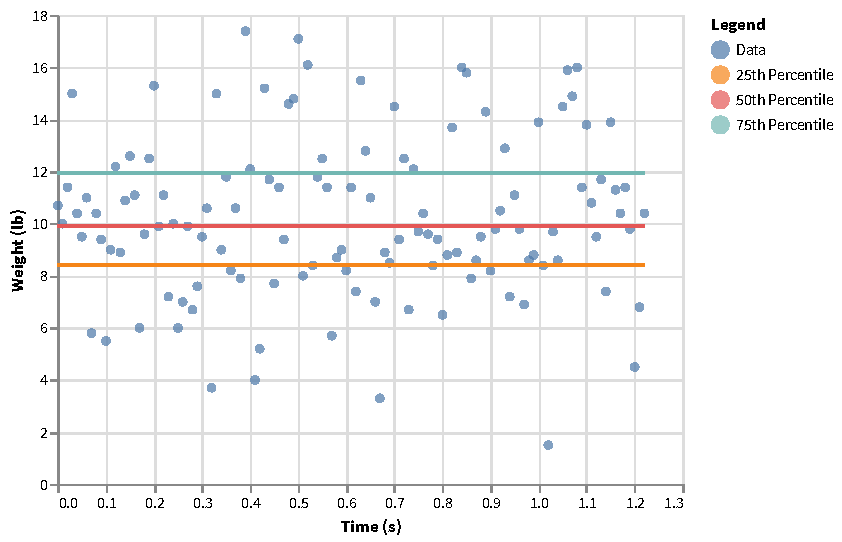
\includegraphics{chart/00-intro/baseline-quartiles.pdf}
    \caption{Quartiles for Baseline Segment}
    \label{figure.00.baseline.quartiles}
\end{figure}
%%%%%%%%%%%%%%%%%%%%%%%%%%%%%%%%%%%%%%%%%%%%%%%%%%%%%%%%%%%%%%%%%%%%%%%%%%%%%%%%
\begin{figure}
    \centering
    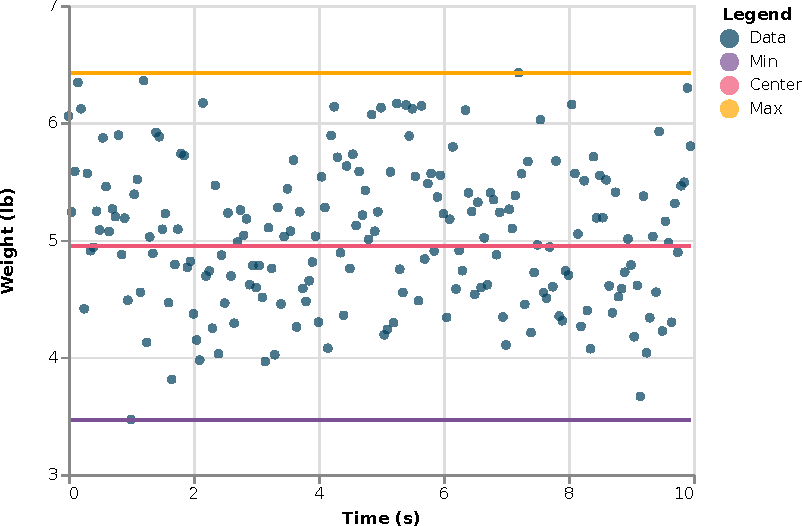
\includegraphics{chart/00-intro/baseline-min-center-max.pdf}
    \caption{Range and Center for Baseline Segment}
    \label{figure.00.baseline.center}
\end{figure}
%%%%%%%%%%%%%%%%%%%%%%%%%%%%%%%%%%%%%%%%%%%%%%%%%%%%%%%%%%%%%%%%%%%%%%%%%%%%%%%%
\begin{figure}
    \centering
    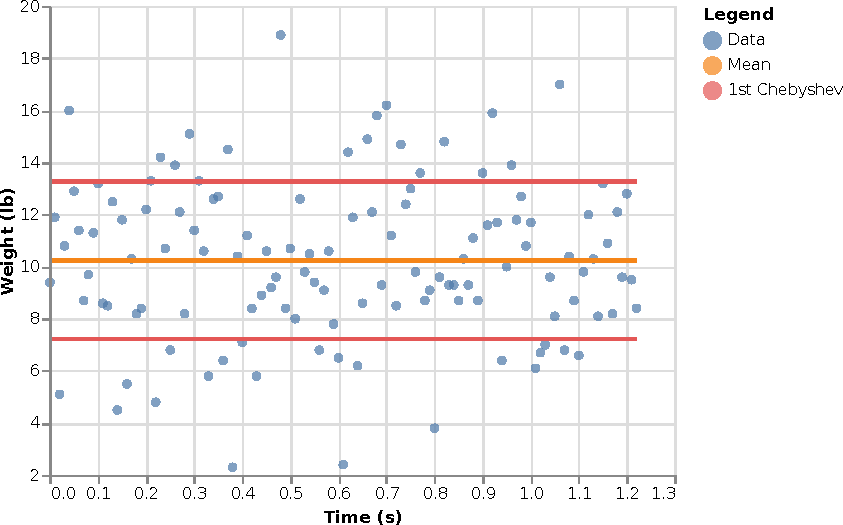
\includegraphics{chart/00-intro/baseline-chebyshev-1.pdf}
    \caption{First Chebyshev Interval for Baseline Segment}
    \label{figure.00.baseline.chebyshev.1}
\end{figure}
%%%%%%%%%%%%%%%%%%%%%%%%%%%%%%%%%%%%%%%%%%%%%%%%%%%%%%%%%%%%%%%%%%%%%%%%%%%%%%%%
\begin{figure}
    \centering
    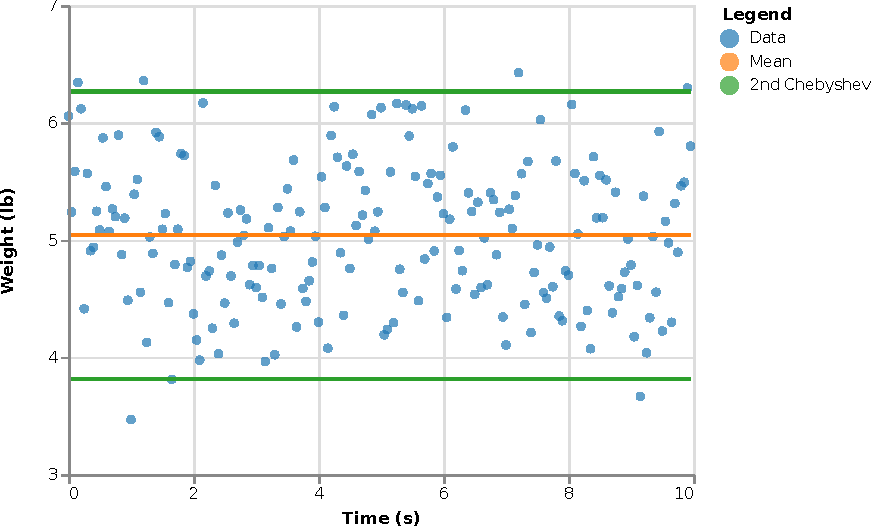
\includegraphics{chart/00-intro/baseline-chebyshev-2.pdf}
    \caption{Second Chebyshev Interval for Baseline Segment}
    \label{figure.00.baseline.chebyshev.2}
\end{figure}
%%%%%%%%%%%%%%%%%%%%%%%%%%%%%%%%%%%%%%%%%%%%%%%%%%%%%%%%%%%%%%%%%%%%%%%%%%%%%%%%
\begin{figure}
    \centering
    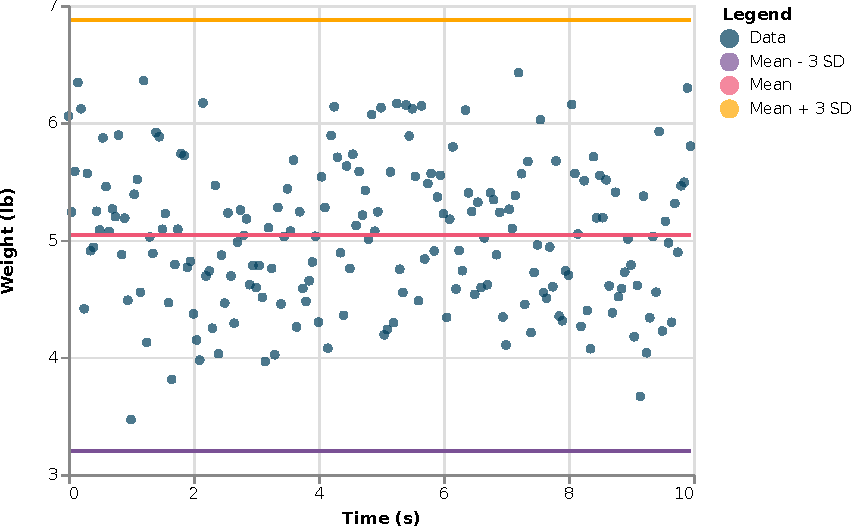
\includegraphics{chart/00-intro/baseline-chebyshev-3.pdf}
    \caption{Third Chebyshev Interval for Baseline Segment}
    \label{figure.00.baseline.chebyshev.3}
\end{figure}
%%%%%%%%%%%%%%%%%%%%%%%%%%%%%%%%%%%%%%%%%%%%%%%%%%%%%%%%%%%%%%%%%%%%%%%%%%%%%%%%
\begin{figure}
    \centering
    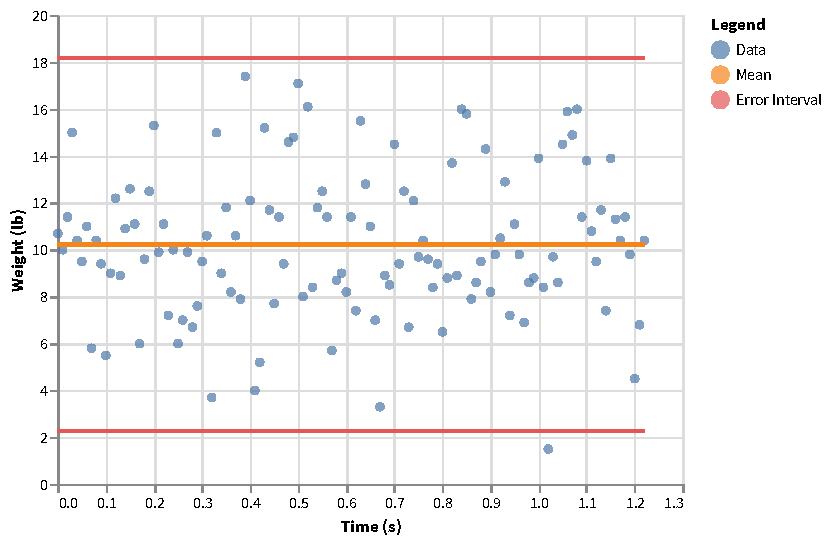
\includegraphics{chart/00-intro/baseline-error-interval.pdf}
    \caption{Error Interval for Baseline Segment}
    \label{figure.00.baseline.interval}
\end{figure}
%%%%%%%%%%%%%%%%%%%%%%%%%%%%%%%%%%%%%%%%%%%%%%%%%%%%%%%%%%%%%%%%%%%%%%%%%%%%%%%%
\section{Your Data}
%%%%%%%%%%%%%%%%%%%%%%%%%%%%%%%%%%%%%%%%%%%%%%%%%%%%%%%%%%%%%%%%%%%%%%%%%%%%%%%%
Your data also consist of two files:
\begin{itemize}
    \item \texttt{weight.tsv}
    \item \texttt{velocity.tsv}
\end{itemize}
However, the ``theoretical'' values for each section are different. See Table \ref{table.00.theoretical.v01} and Table \ref{table.00.theoretical.v02} for specific details.
%%%%%%%%%%%%%%%%%%%%%%%%%%%%%%%%%%%%%%%%%%%%%%%%%%%%%%%%%%%%%%%%%%%%%%%%%%%%%%%%
\begin{table}
    \centering
    \begin{tabular}{|l|r|}
        \hline
        \textbf{Name} & \textbf{Value} \\
        \hline
        Weight 1 & 88 lb \\
        Weight 2 & 160 lb \\
        \hline
        Slope & 13 m/s$^{2}$ \\
        Intercept & 4 m/s \\
        \hline
    \end{tabular}
    \caption{Theoretical values for section V01}
    \label{table.00.theoretical.v01}
\end{table}
%%%%%%%%%%%%%%%%%%%%%%%%%%%%%%%%%%%%%%%%%%%%%%%%%%%%%%%%%%%%%%%%%%%%%%%%%%%%%%%%
\begin{table}
    \centering
    \begin{tabular}{|l|r|}
        \hline
        \textbf{Name} & \textbf{Value} \\
        \hline
        Mass 1 & 93 lb \\
        Mass 2 & 142 lb \\
        \hline
        Slope & 9 m/s$^{2}$ \\
        Intercept & 2 m/s \\
        \hline
    \end{tabular}
    \caption{Theoretical values for section V02}
    \label{table.00.theoretical.v02}
\end{table}
%%%%%%%%%%%%%%%%%%%%%%%%%%%%%%%%%%%%%%%%%%%%%%%%%%%%%%%%%%%%%%%%%%%%%%%%%%%%%%%%
\section{Your Lab Report}
%%%%%%%%%%%%%%%%%%%%%%%%%%%%%%%%%%%%%%%%%%%%%%%%%%%%%%%%%%%%%%%%%%%%%%%%%%%%%%%%
There is no written lab report submission for this activity. However, you have to \textbf{submit a spreadsheet file} with your work, which \textbf{will be graded}. Submissions are done via Canvas.

For part 1, your spreadsheet should include the following:
\begin{enumerate}
    \item ...
\end{enumerate}
For part 2, your spreadsheet should include the following:
\begin{enumerate}
    \item ...
\end{enumerate}
The spreadsheet is due on \textbf{Monday, September 10}.